\chapter{Implementation}\label{chap:impl}

% \begin{guidance}
% This chapter may be called something else\ldots but in general
% the idea is that you have one (or a few) ``meat'' chapters which
% describe the work you did in technical detail.
% \end{guidance}

\prechapter{%
    I will describe the structure of LT4LA: a DSL (domain specific language)
    \textbf{library} written in OCaml that transpiles to OCaml. I will explain
    the features of its core language and show how readable (equational and
    algebraic expressions) and easy to reason about linear algebra programs
    can be elaborated into memory-efficient ones in the core language that are
    then checked for safety (with respect to aliasing, read/write permissions,
    memory allocation, re-use and de-allocation). Finally, I will explain how
    such programs can be transpiled to OCaml code that is not obviously safe.
    Although I refer to OCaml-specific features of the type checker and
    transpiler, I believe the ideas described in this chapter can easily be
    implemented in other languages and are also general enough to transpile to
    other back-end languages, such as C or Fortran.
}%

\section{Structure of LT4LA}\label{sec:structure_lt4la}

LT4LA follows the structure of a typical compiler for a (E)DSL\@. From the
start, I made a concerted effort to (1) write pure-functional code (typically
using a monadic-style) which helped immensely with modularity and debugging
when tests showed errors (2) produce readable, useful and precise
error-messages in the hope that someone who did not understand linear types
could still use LT4LA (3) write tests and set-up continuous-integration for all
non-trivial functions so that I could spot and correct errors that were not
caught by OCaml's type system whenever I implemented new features or refactored
my code.

\begin{enumerate}

    \item \textbf{Parsing}. A generated, LR(1) parser parses a text file into a
        syntax tree. I tried to mimic OCaml syntax modulo a few extensions and
        keywords so that it is familiar and thus easy to pick-up for OCaml
        users. In general, this part will vary for different languages and can
        also be dealt with using combinators or syntax-extensions (the EDSL
        approach) if the host language offers such support .

    \item \textbf{Desugaring}. The syntax tree is then desugared into a
        smaller, more concise, abstract syntax tree. This allows for the type
        checker to be simpler to specify and easier to implement. 

    \item \textbf{Matrix Expressions} are also desugared into the abstract
        syntax tree through simple, yet effective pattern-matching.

    \item \textbf{Type checking}. The abstract syntax tree is explicitly typed,
        with some inference to make writing typical programs more convenient.

    \item \textbf{Code Generation}. The abstract syntax tree is translated into
        OCaml, with a few `optimisations' to produce more readable code. This
        process is type-preserving: LT4LA's type system is embedded into
        OCaml's (Figure~\ref{fig:type_grammar}), and so the OCaml type checker
        acts as a sanity check on the generated code.

    \item \textbf{Executable Artifacts}. A transpiler and a REPL are the main
        artifacts produced for this thesis. For evaluation, I implemented
        Kalman filters in Owl, LT4LA and CBLAS/LAPACKE and a benchmarking
        program to measure execution times.

    \item \textbf{Tests}. As mentioned before, almost all non-trivial functions
        have tests to check their behaviour. The output of the transpiler was
        also tested by having the build system generate OCaml code at compile
        time, which in turn could then be compiled and tested like handwritten
        OCaml code.

\end{enumerate}

\section{Core Language}\label{sec:core_lang}

A full description of the core language can be found in
Appendix~\ref{chap:ott_spec}. For convenience, I have reproduced its type
grammar and its translation into OCaml in Figure~\ref{fig:type_grammar}.  The
point of LT4LA is to keep the same values and types we are familiar with from
OCaml, but \emph{restrict their usage}. LT4LA's core language's main features
are: intuitionistic values, value-restriction, fractional-capabilities
(inferrable at call sites), if-expressions and recursion.

\begin{figure}[tp]
    \centering
    \begin{minipage}{.3\textwidth}
        \centering
        \begin{grammar}
            <f> ::= `'
            \alt <fc>
            \alt `Z'
            \alt `S' <f>

            <t> ::= `'
            \alt `unit'
            \alt `bool'
            \alt `int'
            \alt `elt'
            \alt <f> `arr'
            \alt <f> `mat'
            \alt `!' <t>
            \alt \synt{$\forall$} <fc.> <t>
            \alt <t> \lit{$\otimes$} \synt{$t'$}
            \alt <t> \lit{$\multimap$} \synt{$t'$}
        \end{grammar}
    \end{minipage}
    \begin{minipage}{.3\textwidth}
        \centering
        \begin{minted}[fontsize=\small, linenos]{ocaml}
module Arr =
  Owl.Dense.Ndarray.D

type z = Z
type 'a s = Succ

type 'a arr =
  A of Arr.arr
  [@@unboxed]

type 'a mat =
  M of Arr.arr
  [@@unboxed]

type 'a bang =
  Many of 'a
  [@@unboxed]
        \end{minted}
    \end{minipage}
    \begin{minipage}{.3\textwidth}
        \begin{align*}
            [\![ f\!c ]\!] &= \texttt{'fc} \\
            [\![ \textbf{Z} ]\!] &= \texttt{z}\\
            [\![ \textbf{S} \, f ]\!] &= [\![ f ]\!]\, \texttt{s}\\
            [\![ \textbf{unit} ]\!] &= \texttt{unit}\\
            [\![ \textbf{bool} ]\!] &= \texttt{bool}\\
            [\![ \textbf{int} ]\!] &= \texttt{int}\\
            [\![ \textbf{elt} ]\!] &= \texttt{float}\\
            [\![ f\, \textbf{arr} ]\!] &= [\![ f ]\!]\, \texttt{arr}\\
            [\![ f\, \textbf{mat} ]\!] &= [\![ f ]\!]\, \texttt{mat}\\
            [\![ \textbf{!} \, t ]\!] &= [\![ t ]\!]\, \texttt{bang}\\
            [\![ \forall f\!c.\, t ]\!] &= [\![ t ]\!]\\
            [\![ t \otimes t' ]\!] &= [\![ t ]\!] \texttt{*} [\![ t' ]\!]\\
            [\![ t \multimap t' ]\!] &= [\![ t ]\!] \rightarrow [\![ t' ]\!]
        \end{align*}
    \end{minipage}
    \caption{Type grammar of LT4LA (left) and my translation of it
        into OCaml (right).}\label{fig:type_grammar}
\end{figure}

\subsection{Intuitionistic Values}

To make LT4LA a usable DSL, I needed a way of allowing values to either never
be used or be used more than once. For this, I added the \mbox{!-constructor}
at the type-level of the DSL and its corresponding introduction (the
\ltfla{Many}-constructor) and elimination (the \ltfla{let Many <id> = .. in ..
} destructor) forms at the term-level of the DSL.  The idea behind the
\mbox{!-constructor} is that a value of that type uses no `resources'
(linearly-typed expressions). To start off with, it is enough to say that
anything which can be passed around by copying, will have a \mbox{!-type}. This
includes integers, elements and booleans. So \ltfla{3 : !int} and \ltfla{3. +.
4. : !elt}. However, all bindings are still linear by default, so to emulate
intuitionism, I desugar \ltfla{let !x = <exp> in <body>} to \ltfla{let Many x =
<exp> in let Many x = Many (Many x) in <body>} (similarly for function argument
bindings). The reader can check (using the rules in
Appendix~\ref{chap:ott_spec}) that this has the effect of moving \ltfla{x : !t}
from the linear to the intuitionistic environments, only if \ltfla{<exp> : !t}.

However, just that desugaring alone is not enough to prevent a user from taking
an array or matrix and moving it into the intuitionistic environments. Why?
There are certain situations in which we \emph{should not} use the \ltfla{Many}
constructor.  Consider the following code: \ltfla{let Many x = Many (array 5)
in <body>}; the expression \ltfla{array 5} uses no linearly-typed variables
from the environment. Although we could just reject types of the form
\ltfla{!(_ arr)} to fix this simple example, what about pairs \ltfla{let Many
xy = Many (3, array 5) in <body>}?  Ad-hoc pattern matching on the type cannot
account for all possible situations. With the last case, we can use \ltfla{xy}
as many times as we would like, destruct the pair to get the second component
and thus create \emph{distinct} read-write aliases to the same array.  Alas,
now arrays can be used intuitionistically and all the benefits of linearity are
lost.  Or are they?

\subsection{Value-Restriction}

Not quite, but to understand how we can fix this problem, we need to question
an assumption left implicit up until this point: what does \ltfla{Many} even
mean in the DSL? How is it translated to OCaml? What is the OCaml runtime
behaviour of the DSL's \ltfla{Many}-constructor? One option is to go down the
C++ route and make \ltfla{Many} behave like a \ltfla{shared_ptr} and act as a
runtime reference-count for arrays. I chose to not go for this option because
it went against the \emph{explicitness} and \emph{predictability} that C and
Fortran have. It would make analysing when and what is allocated and freed more
like the higher-level languages I was trying to move away from.

My aim is to show linear types are simple to understand and apply, enough so
that they can be grafted (in a limited way) on to existing languages as a
\emph{library}. In that spirit, the simplest thing that the DSL's
\ltfla{Many}-constructor can mean in the OCaml runtime is \emph{nothing}.
LT4LA's !/\ltfla{Many} constructors are translated into OCaml
\ltfla{bang}/\ltfla{Many} constructors declared as \ltfla{type 'a bang = Many
of 'a [@@unboxed]}.  The \emph{unboxed} annotation means that the type and its
constructor only exist for the purpose of type checking in OCaml; \emph{the
OCaml runtime representation of values of type \ltfla{'a} and \ltfla{'a bang}
is exactly the same}.

With this understanding, our problem is that arrays and matrices are unlike
other values such as integers and elements because (under the OCaml hood)
calling a function with an array argument copies a \emph{pointer} to the array
rather than the array itself. So, we can start making a distinction,
\emph{defining} elements, integers, booleans, intuitionistic variables, units
and lambda-expressions that capture no linear variables as \emph{values} (since
they cannot break referential-transparency) and anything else (arrays,
matrices, expressions which can be reduced, such as function application and
if-expressions) as not being `values'. If this sounds familiar, it is because
this is the same \emph{value-restriction} `trick' from the world of polymorphic
types applied to linearity instead. We then have the rule that in LT4LA, we can
only use \ltfla{Many} on expressions that are defined to be \emph{values} and
\emph{use no linear variables}.

\subsection{Fractional-Capabilities and Inference}

I started off with linearity and showed how it helps a programmer keep track
of memory allocation and deallocation, and then demonstrated how to add
intuitionism for the only values we wish to be intuitionistic. I will now
explain how I enforce safe aliasing and read/write permissions.

Array and matrix types are parameterised by
\emph{fractional-capabilities}~\cite{boyland}.  A fraction of 1 ($2^0$)
represents complete ownership of a value. Creating an array gives you ownership
of it; the function \ltfla{array : !int --o z arr} (where \ltfla{z} represents
`0').  Once you have ownership of an array, you can free it: \ltfla{free : z
arr --o unit}.  Importantly, because a linear value may only be used once, the
array just freed is \emph{out of scope} for following expressions,
\textbf{preventing use-after-free}.  Ownership also enables you to write to the
array: \ltfla{set : z arr --o !int --o !elt --o z arr} (the syntax \ltfla{w[i]
:= j} is just sugar for \ltfla{set w i j}). Here, linearity prevents accessing
aliases which represented the array \emph{before} the mutation.

Any fraction less than 1 (for simplicity, limited to $2^{-k}$ in this system,
for a positive integer $k$) represents read-only access. So, the \ltfla{'x}
represents a natural number (either a zero \ltfla{z}, variable \ltfla{'x} or a
successor (+1) of a natural number). Hence, you can read from (index) any array
\ltfla{get : 'x .  'x arr --o !int --o 'x arr * !elt} (the syntax \ltfla{let !v
<- w[i]} is just sugar for \ltfla{let (w, !v) = get _ w i}). In general, a
left-arrow \ltfla{<-} signifies transparent rebinding with returned values: it
means a program can \emph{appear} to use a variable multiple times, important
for keeping LT4LA usable and readable. The underscore is how a programmer tells
the compiler to automatically \emph{infer} the correct fractional-capability
based on the other arguments passed to the function. In conjunction with the
requirement that function declarations need type-annotations for their
arguments, \textbf{this allows fractional-capabilities to be \emph{correctly
inferred} in \emph{any} LT4LA expression}.

Fractions exist to provide both safe aliasing and read/write permissions, via
the primitives \ltfla{share : 'x . 'x arr --o ('x s) arr * ('x s) arr} and
\ltfla{unshare: 'x .  ('x s) arr --o ('x s) arr --o 'x arr}.  For the former,
the two arrays returned (which are just aliases of the given array) can now
only be read from and not written to. If you want to write to this array, you
must use the latter to combine other read-only aliases until you are left with
only one value of type \ltfla{z arr}, guaranteeing no other aliases exists.

Given this set-up, a programmer now \emph{statically} has \emph{perfect}
information about aliasing and ownership of values in the program. They can
only write to or free an array only when they own it; ownership guarantees no
other aliases exist. In Figure~\ref{fig:ltfla_kalman}, I show how this perfect
information can be used to write more readable (equational and algebraic) code
using easy to reason about, value-semantic expressions whose \emph{intensional}
behaviour and assumptions (regarding aliasing, read/write permissions and
memory allocation, re-use and de-allocation) are also explicitly and precisely
described and \emph{automatically checkable}. Now the programmer need not
resort to manually figuring out and inserting \texttt{noalias} annotations and
worrying about what variables can and cannot be written to, re-used or freed;
instead they can let the loyal and tireless compiler do the heavy lifting.

\subsection{If-Expressions}

An if-expression's condition may evaluate either way during execution, so a
programmer must guarantee that both branches use the same set of linear
variables. Writing the type checker in a pure-functional monadic style paid off
here because I could now sandwich monadic values with state adjustments either
side of it. Given two monadic values that represented type checking two
branches of an if-expression, I could use the code in
Figure~\ref{fig:same_resources} to easily save, reset and compare the state
either side of running those monadic values.

\begin{figure}[tp]
    \begin{minted}[fontsize=\small]{ocaml}
let same_resources (wf_a, loc_a) (wf_b, loc_b) =
  let open Let_syntax in
  (* Save state *)
  let%bind {used_vars=prev; env=old_env; _} as state = get in
  (* Reset, run a, save state *)
  let%bind () = put { state with used_vars = empty_used } in
  let%bind res_a = wf_a in
  let%bind {used_vars=used_a; _} as state = get in
  (* Reset, run b, save state *)
  let%bind () = put { state with used_vars = empty_used; env = old_env } in
  let%bind res_b = wf_b in
  let%bind {used_vars=used_b; _} as state = get in
  (* Check if same resources *)
  let keys_a, keys_b = (* convert to (used_a, used_b) to sets *) in
  if Set.equal keys_a keys_b then
    (* merge used_vars and used_b environments *)
  else
    (* report differences *)
    \end{minted}

    \caption{Implementation of same\_resources helper method for type checking
        if-expressions. Note the monadic style helped compose computations that
        affected the type checker's state in a simple manner.}\label{fig:same_resources}

\end{figure}

\subsection{Functions and Recursion}

A non-recursive function may be used more than once if it does not refer to any
linear variables from the surrounding scope. So, we can desugar something like
\ltfla{let x = 3 in let !f (y : !int) = x + y in <body>} to \ltfla{let x = 3 in
let Many f =  Many (fun y : !int -> x + y) in  <body>}.  Recursion is slightly
more complicated: we can desugar the factorial function
(Figure~\ref{fig:ltfla_factorial}) to \ltfla{let Many f = fix (f, x : !int, if
(*..*) : !int) in <body> }. However, \ltfla{fix}, like \ltfla{Many}, must also
not use any linear variables from its surrounding scope, because a
recursive function may evaluate its body multiple times.

\begin{landscape}
    \begin{figure}[p]
    \centering
    \begin{minipage}{1.47\textheight}
    \inputminted[linenos, fontsize=\footnotesize]{fortran}{kalman.f90}
    \end{minipage}
    \caption{Kalman filter in Fortran 90.}\label{fig:fortran_kalman}
    \end{figure}
\end{landscape}

\section{Matrix Expressions}\label{sec:matrix_exps}

We have now arrived at an extended application of linear types. I will show how
we can apply the ability to automatically check aliasing, read/write
permissions, memory allocation, re-use and deallocation, to the domain of
matrix-expression compilation (automatically generating code like
Figure~\ref{fig:fortran_kalman} from mathematical expressions like
Figure~\ref{fig:maths_kalman}).

In Figure~\ref{fig:fortran_kalman}, we see the difficulty of efficiently
implementing a \emph{Kalman filter}~\cite{kalman}, a powerful set of equations
(Figure~\ref{fig:maths_kalman}) applicable to a wide variety of problems. From
the comments, we see that every variable is annotated with the matrix
expression that it will hold at some point during the computation (an
equivalent alternative, say in C++, could be to have a meaningful name for each
step and manually keep track of which names alias the same location).

\begin{figure}[tp]
    \begin{align*}
        \mu' &= \mu + \Sigma H^T (R + H \Sigma H^T)^{-1} (H \mu - \textrm{data})\\
        \Sigma' &= \Sigma ( I - H^T (R + H \Sigma H^T)^{-1} H \Sigma )
    \end{align*}
    \caption{Kalman filter equations (credit:
    \href{http://matthewrocklin.com/blog/work/2012/11/24/Kalman-Filter}{matthewrocklin.com}).}\label{fig:maths_kalman}
\end{figure}

In contrast, Figure~\ref{fig:ltfla_kalman}, offers the advantages of
\begin{itemize}
    \item aliasing: labelling each step with a different, more meaningful variable name,
    \item easily spotting which resources are being passed in and which are
        allocated for the function (new/copy),
    \item unambiguously seeing \emph{when} and what values are freed or written-over;
\end{itemize}
and have the compiler automatically ensure the safety of each of the above by respectively
\begin{itemize}
    \item making it impossible to refer to values which are no longer usable,
    \item ensuring all values are declared and \emph{initialised} correctly before they are used,
    \item checking values are neither used after they are freed/written-over \emph{nor} leaked.
\end{itemize}

Indeed, an inexperienced programmer could take the  na\"ive approach of just
copying sub-expressions by default and then letting the compiler tell them
which copies are never used and removing them systematically until their
program type checks.  While it is not quite a black-box, push-button
compilation of an expression, I would argue it is just as easy (if not easier)
to learn how to work with as Rust's borrow checker.

\begin{figure}[tp]
    \inputminted[linenos, fontsize=\small]{ocaml}{../test/examples/kalman.lt}
    \caption{Kalman filter in LT4LA. In contrast with the Fortran
        (Figure~\ref{fig:fortran_kalman}) or C (Figure~\ref{fig:cblas_kalman})
        implementations, this one is readable (equational and algebraic),
        using easy to reason about, value-semantic expressions. In addition to
        that, its \emph{intensional} behaviour and assumptions (regarding
        aliasing, read/write permissions and memory allocation, re-use and
        de-allocation) are also explicitly and precisely described and
        \emph{automatically checkable}.}\label{fig:ltfla_kalman}
\end{figure}

\subsection{Elaboration}

All of the syntax in Figure~\ref{fig:ltfla_kalman} can be unambiguously
desugared \emph{before} type checking, through fairly simple pattern matching.
Matrix expression compilation is well-trodden territory in
academia~\cite{rocklin_thesis, fabregat_thesis, gunnels_flame, linnea, taco}
but this is, to my knowledge, the \textbf{first type-based approach} to it.

An overview of the translations are in Figure~\ref{fig:mat_patterns}; details
about choosing between `symm' or `gemm' are omitted for brevity. Before
settling on this approach, I tried implementing a more general type-directed,
nested matrix expression compiler; I will now highlight some of the
difficulties inherent in the problem.

\begin{figure}[tp]
    \begin{minted}[fontsize=\small]{ocaml}
let x <- [| y |] in ..              ==> let (y,x) = copyM_to _ y x in ..
let x <- new [| y |] in ..          ==> let (y,x) = copyM _ y in ..
let x <- [| a*b + c |] in ..        ==> let x <- [| 1.*a*b + 1.*c |] in ..
let x <- [| i*a*b + j*c |] in ..    ==> let ((a,b), c) = (* BLAS *) in ..
let x <- new (m, n) [| a*b |] in .. ==> let c = matrix m n in
                                        let x <- [| 1.*a*b + 0.*c |] in ..
    \end{minted}
    \caption{Syntactic translations of matrix expressions to linearly-typed
        matrix functions. Further annotations on the matrix variables
        (\ltfla{sym} or \ltfla{^T}) determine which BLAS routine is called and
        what parameters it is passed.}\label{fig:mat_patterns}

\end{figure}

One of the first hurdles I encountered was compositionality: to compile $AB +
C$ it is typically better to use a BLAS routine directly rather than first
compiling $A$, then $B$, then adding a call to multiply them, then compiling
$C$ and finishing with a call to add the results.

Another compositionality problem is that a call to a linear function does not
just return a result, but a sequence of re-bindings which dictate which
variables are still usable (in scope).  As such, to compile an expression, you
need to provide a CPS-style function of type $var \rightarrow exp$ representing
how you would use a variable representing the result in the rest of the
computation.

However, the type of that variable also determines how you can use it: can you
write to it or must you copy it? This information depends on how the expression
representing the variable was elaborated and adds to the complexity of the
pattern-matching.

Copying leads us into dealing with temporaries: do you first allocate all
temporaries in new matrices (SSA-style) and then analyse dimensions to figure
out which slots of memory can be re-used via copy coalescing? Or do you try and
infer the live ranges of available resources from the environment as you go?
Can, and should, you type arrays and matrices (or $n$-dimensional tensors) as
the same?

Adding in more and more considerations, the problem starts to resemble register
allocation: there are registers of different types and sizes, many
(non-orthogonal) instructions to choose from, a cost model to take into account
all whilst trying to balance the number of registers in use and the number of
instructions emitted.

\section{Code Generation}

Code generation is a straightforward mapping from core LT4LA constructs to
OCaml constructs, with the addition of \ltfla{Many} constructors to wrap
integer, element and boolean literals.

To make the code produced readable, I added a few `optimisations', to the
compiler, to `re-sugar' some of the constructs translated where appropriate.
Almost all of them involved the erasing the \mbox{!-eliminator} which is not needed in
regular, intuitionistic OCaml. So, we can simply replace any expression of
the form:

\begin{itemize}

    \item \ltfla{let xy, z = <exp> in let x,y = xy in <body>} with
        \ltfla{let (x,y), z = <exp> in <body>}, 

    \item \ltfla{let Many x = x in let Many x = Many (Many x) in <body>} with
        \ltfla{<body>},

    \item \ltfla{let Many x = <exp> in let Many x = Many (Many x) in <body>} with
        \ltfla{let x = <exp> in <body>},

    \item \ltfla{let Many x = Many <exp> in <body>} with \ltfla{let x = <exp> in <body>},

    \item \ltfla{let Many f = fix (f, x, .., <exp>, ..) in <body>} with
        \ltfla{let rec f x = <exp> in <body>}.

\end{itemize}

The end result is visible in Figures~\ref{fig:ocaml_sumarray}
and~\ref{fig:ocaml_kalman}:  (surprisingly beautiful) OCaml code that is not
obviously safe, as promised at the start of the chapter.

\begin{figure}[tp]
    \centering
    \begin{minted}[linenos, fontsize=\small]{ocaml}
let rec f i n x0 row =
  if Prim.extract @@ Prim.eqI i n then (row, x0)
  else
    let row, x1 = Prim.get row i in
    f (Prim.addI i (Many 1)) n (Prim.addE x0 x1) row
in
f
    \end{minted}
    \caption{Recursive OCaml function for a summing over an array, generated (at
        \emph{compile time}) from the code in Figure~\ref{fig:ltfla_sumarray},
        passed through \texttt{ocamlformat} for presentation.}\label{fig:ocaml_sumarray}

\end{figure}

It is clear that both Figures~\ref{fig:fortran_kalman}
and~\ref{fig:ocaml_kalman} are realisations of a concise, linearly-typed Kalman
filter~\ref{fig:ltfla_kalman} \emph{specification} that describes the intensional
behaviour and assumptions (with respect to read/writes permissions, memory
management and aliasing) of the program and the BLAS primitives it uses \textbf{more
accurately} than a Fortran, C or OCaml implementation could.

\begin{figure}[p]
    \begin{minted}[linenos, fontsize=\footnotesize]{ocaml}
let kalman sigma h mu r_1 data_1 =
  let h, _p_k_n_p_ = Prim.size_mat h in
  let k, n = _p_k_n_p_ in
  let sigma_h = Prim.matrix k n in
  let (sigma, h), sigma_h =
    Prim.symm (Many true) (Many 1.) sigma h (Many 0.) sigma_h
  in
  let (sigma_h, h), r_2 =
    Prim.gemm (Many 1.) (sigma_h, Many false) (h, Many true) (Many 1.) r_1
  in
  let (h, mu), data_2 =
    Prim.gemm (Many 1.) (h, Many false) (mu, Many false) (Many (-1.)) data_1
  in
  let h, new_h = Prim.copy_mat_to h sigma_h in
  let r_2, new_r = Prim.copy_mat r_2 in
  let chol_r, sol_h = Prim.posv new_r new_h in
  let chol_r, sol_data = Prim.potrs chol_r data_2 in
  let () = Prim.free_mat chol_r in
  let h_sol_h = Prim.matrix n n in
  let (h, sol_h), h_sol_h =
    Prim.gemm (Many 1.) (h, Many true) (sol_h, Many false) (Many 0.) h_sol_h
  in
  let () = Prim.free_mat sol_h in
  let h_sol_data = Prim.matrix n (Many 1) in
  let (h, sol_data), h_sol_data =
    Prim.gemm (Many 1.) (h, Many true) (sol_data, Many false) (Many 0.) h_sol_data
  in
  let mu, mu_copy = Prim.copy_mat mu in
  let (sigma, h_sol_data), new_mu =
    Prim.symm (Many false) (Many 1.) sigma h_sol_data (Many 1.) mu_copy
  in
  let () = Prim.free_mat h_sol_data in
  let h_sol_h_sigma = Prim.matrix n n in
  let (sigma, h_sol_h), h_sol_h_sigma =
    Prim.symm (Many true) (Many 1.) sigma h_sol_h (Many 0.) h_sol_h_sigma
  in
  let sigma, sigma_copy = Prim.copy_mat_to sigma h_sol_h in
  let (sigma, h_sol_h_sigma), new_sigma =
    Prim.symm (Many false) (Many (-1.)) sigma h_sol_h_sigma (Many 1.) sigma_copy
  in
  let () = Prim.free_mat h_sol_h_sigma in
  ((sigma, (h, (mu, (r_2, sol_data)))), (new_mu, new_sigma)) )
in
kalman
    \end{minted}
    \caption{OCaml code for a Kalman filter, generated (at \emph{compile time})
        from the code in Figure~\ref{fig:ltfla_kalman}, passed through
        \texttt{ocamlformat} for presentation.}\label{fig:ocaml_kalman}

\end{figure}

\subsection{Build System}

So once you have written your memory-optimised program with all the features
and support provided by LT4LA and made it produce well-typed, compilable OCaml
code, the question then becomes, how to use this code. This process will vary
across ecosystems, but within OCaml, the new build system on the block
\emph{Dune} has support for generating, compiling and linking OCaml modules at
\emph{compile time} (Figure~\ref{fig:build}). Indeed, this is how I have written
tests and benchmarks for programs produced by LT4LA from within OCaml. In
particular, I can use my linearly-typed Kalman filter implementation just like
and with any other OCaml function.

\begin{figure}[t]
    \centering
    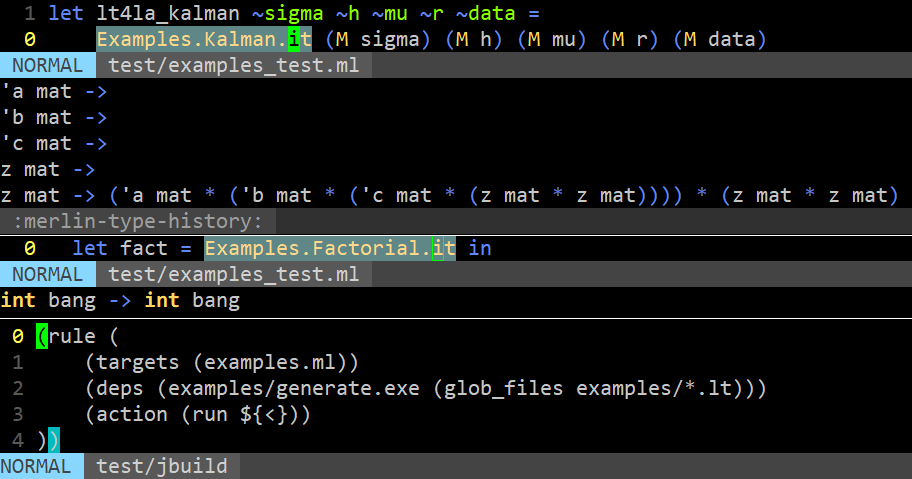
\includegraphics[width=\textwidth]{impl_build}
    \caption{Using LT4LA functions from OCaml with the Dune
        build system.}\label{fig:build}
\end{figure}

Generating code at compile time has two advantages. First, it avoids runtime
overhead. Second, it catches interface and \textbf{relevant implementation
changes} between the generated code and the code that uses it.  The second
advantage is \emph{another benefit} of \emph{embedding} LT4LA's type system
inside of OCaml's. Relevant implementation changes are caught because LT4LA's
types express some of the intensional behaviour and assumptions of its
programs.

I suspect that this approach will be very valuable to not just \emph{users} of
libraries such as Numpy or Owl, but also their \emph{implementors}: library
functions which present a safe, value-semantic interface but use unsafe,
mutating operations on the inside could now be expressed using LT4LA and gain
\textbf{safety, value-semantics and automatic checking for their implementations}.

\clearpage%
\section{Summary}

I explained how a few core features -- linearity, the \ltfla{Many}
constructor, value-restriction, fractional-capabilities with inference,
if-expressions and recursive functions -- are enough to \emph{statically
capture and automatically check} aliasing, read/write permissions, memory
allocation, re-use and deallocation of non-trivial linear algebra programs. I
also demonstrated that simple pattern-matching and desugaring provides the
potential for a \textbf{new, \emph{type-directed}} approach to matrix expression
compilation. Lastly I have shown that it is possible to use these features with
\emph{existing} languages and frameworks.\footnote{As mentioned in the previous
chapter, if the host language supports \emph{syntax-extensions}, like PPX
for OCaml, it is possible to construct LT4LA expressions \emph{from within} the
host language.}

